\documentclass[tikz,border=5mm]{standalone}
\usepackage{pgfplots}
\usepackage{amsmath}
\pgfplotsset{compat=1.18}

\definecolor{plotblue}{RGB}{65, 105, 225}
\definecolor{dotred}{RGB}{220, 20, 60}
\definecolor{arrowgreen}{RGB}{0, 100, 0}

\begin{document}
	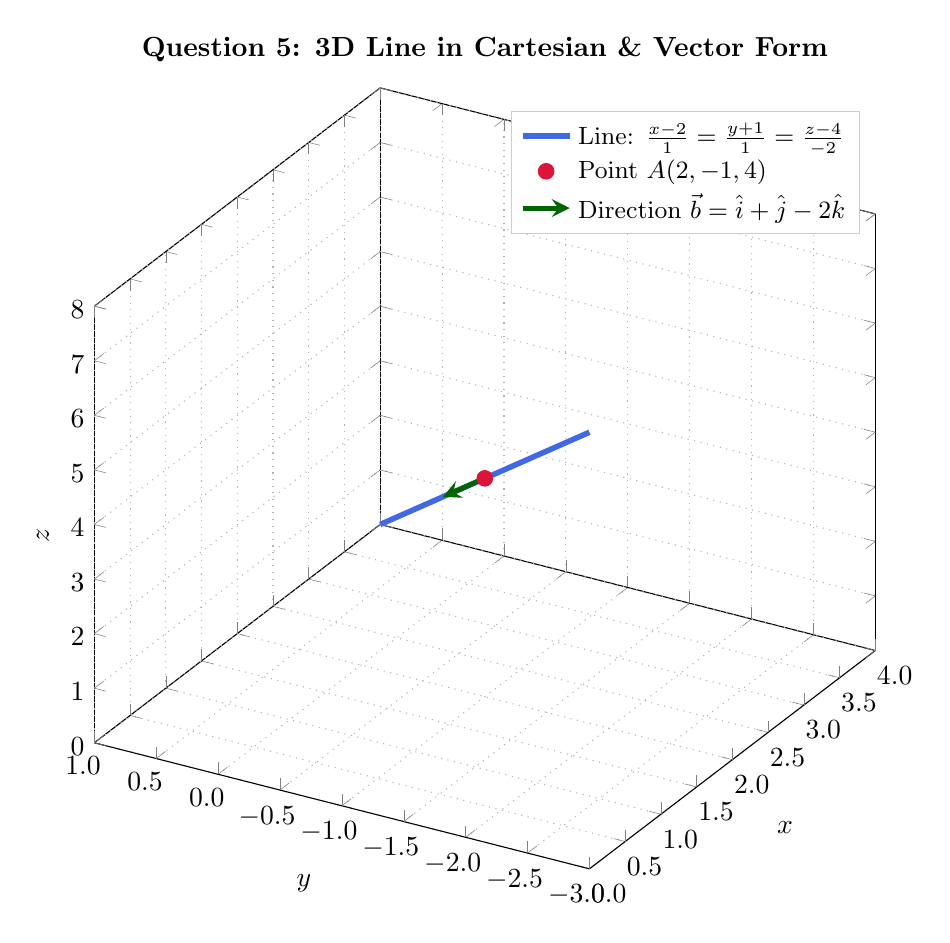
\begin{tikzpicture}
		\begin{axis}[
			width=11.5cm, height=11.5cm,
			view={-60}{30},
			title={\textbf{Question 5: 3D Line in Cartesian \& Vector Form}},
			xlabel={$x$}, ylabel={$y$}, zlabel={$z$},
			xmin=0, xmax=4,
			ymin=-3, ymax=1,
			zmin=0, zmax=8,
			xtick={0.0, 0.5, 1.0, 1.5, 2.0, 2.5, 3.0, 3.5, 4.0},
			xticklabel style={/pgf/number format/fixed, /pgf/number format/precision=1, /pgf/number format/zerofill},
			ytick={-3.0, -2.5, -2.0, -1.5, -1.0, -0.5, 0.0, 0.5, 1.0},
			yticklabel style={/pgf/number format/fixed, /pgf/number format/precision=1, /pgf/number format/zerofill},
			ztick={0, 1, 2, 3, 4, 5, 6, 7, 8},
			grid=both,
			grid style={dotted, gray!60},
			legend cell align={left},
			legend style={at={(0.98,0.97)}, anchor=north east, font=\small, draw=gray!40}
			]
			% 3D Line: (x-2)/1 = (y+1)/1 = (z-4)/(-2) -> from (0,-3,8) to (4,1,0)
			\addplot3[plotblue, line width=2pt] coordinates {(0, -3, 8) (4, 1, 0)};
			\addlegendentry{Line: $\frac{x-2}{1} = \frac{y+1}{1} = \frac{z-4}{-2}$}
			
			% Point A(2, -1, 4)
			\addplot3[only marks, mark=*, mark size=2.8pt, dotred] coordinates {(2, -1, 4)};
			\addlegendentry{Point $A(2, -1, 4)$}
			
			% Direction Vector b = i + j - 2k
			\addplot3[arrowgreen, line width=1.8pt, -{stealth[scale=1.3]}] coordinates {(2, -1, 4) (2.8, -0.2, 2.4)};
			\addlegendentry{Direction $\vec{b} = \hat{i} + \hat{j} - 2\hat{k}$}
		\end{axis}
	\end{tikzpicture}
\end{document}